\documentclass[conference]{IEEEtran}
\usepackage[T1]{fontenc}
\usepackage[utf8]{inputenc}
\usepackage{amsmath,amssymb,graphicx,booktabs,cite}
\usepackage{tikz}
\usetikzlibrary{arrows.meta,positioning}
\usepackage{balance}
\usepackage[hidelinks,breaklinks]{hyperref}
\usepackage{url}
\hypersetup{pdftitle={History-Aware Learning for Task-Aware Cellular Molecular Communication},
 pdfauthor={Ruifeng Zheng}, pdfsubject={Working draft with experimental-data prediction results and a proposed controller},
 pdfkeywords={molecular communication, cellular receivers, FGF2, ERK, history-aware learning}}
\newcommand{\E}{\mathbb{E}}
\newcommand{\Prob}{\mathbb{P}}
\newcommand{\Hist}{\mathcal{H}}
\newcommand{\ind}{\mathbf{1}}
\newcommand{\calA}{\mathcal{A}_{\mathrm{cal}}}
\hyphenation{micro-fluidic micro-fluidics}
\title{History-Aware Learning for Task-Aware\protect\\Cellular Molecular Communication}
\author{\IEEEauthorblockN{Ruifeng Zheng}\IEEEauthorblockA{Deutsche Telekom Chair of Communication Networks\\TU Dresden, Germany}}
\begin{document}
\maketitle
\pagestyle{plain}
\thispagestyle{plain}

\begin{abstract}
Chemical commands delivered to a living receiver can alter its subsequent response, making the useful state of the receiver depend on both the present signal and its stimulation history. We study this issue using publicly available, experimentally measured FGF2--ERK reporter trajectories rather than artificial bit labels. A provenance-checked pilot contains 606 single-cell trajectories and 53,998 measurements. Entire sustained and periodic-pulse conditions are used for training, single-pulse conditions for validation, and mixed-pulse conditions for testing. A causal-history ridge predictor achieves a condition-equal root mean squared error of 0.026817 at a 10-minute horizon, compared with 0.029229 for a current-input/current-response/clock baseline, an 8.25\% relative reduction. The corresponding two-minute gain is small. An exploratory within-cell comparison does not consistently establish an additional history effect after matching the current reporter and slope. We then formulate task-dependent receiver readiness and a constrained receding-horizon controller for repeated chemical commands. This control framework is a proposed specification, not an evaluated policy. The present evidence supports a limited forecasting result and motivates prospective tests of receiver reuse; it establishes neither a new biological mechanism nor improved task reliability or molecular economy.
\end{abstract}

\begin{IEEEkeywords}
Molecular communication, cellular receivers, chemical signaling, history-aware learning, FGF2, ERK, model predictive control.
\end{IEEEkeywords}

\begin{center}
\footnotesize\textit{Working draft, 4 October 2026. Experimental-data prediction pilot completed; task-control experiments pending.}
\end{center}

\section{Introduction}
An application of molecular communication (MC) can require a chemical signal to produce a specified response in a living cell. In this setting, successful reception is more than recovering a symbol: the receiver must execute the requested response at the right time. A previous exposure may influence the next response through transport persistence, receptor dynamics, intracellular feedback, or changes in cellular state. For a sequence of commands, an operational question is therefore when the receiver can be used again, and at what chemical and temporal cost.

This question should be grounded in a measurable application. Experimental signaling data offer recorded chemical perturbations and individual cellular responses, but they do not automatically constitute a calibrated communication link. The present study uses FGF2 stimulation of PC-12 cells and ERK activity measured with a FRET reporter. The source study connects temporal perturbations to signaling architecture \cite{blum2019}; earlier experiments connect ERK stimulation patterns with cellular outcomes \cite{ryu2015}. Here the recorded reporter is treated as a continuous receiver output. No communication alphabet or cell-fate label is retroactively assigned to the data.

Learning can help summarize a partially observed receiver, but a generic learning-based controller would be a weak novelty claim. Existing studies already address semantic learning in MC \cite{cheng2024,cai2025}, chemical feedback control in mammalian cells \cite{postiglione2018}, and deep model predictive control of cellular expression \cite{lugagne2024}. MC-specific work also addresses signaling control and refractory behavior \cite{barros2020}, adaptive signaling error control \cite{borges2024}, and long-term experimental reuse \cite{scherer2025}. These precedents make a broad claim of first combining learning, biological memory, and reset untenable.

The narrower research question is whether a measured chemical-response history improves prediction beyond accessible present-state information, and whether that additional information can eventually reduce exposure or completion time for \emph{repeated tasks at matched reliability}. A useful result must survive comparisons with current response, slope, protocol time, and a biochemical state estimator receiving the same feedback. It must also separate concentration delivered to the cell from the concentration commanded at the actuator.

This working draft makes three bounded contributions. First, it assembles and audits an experimental input--response pilot with an explicit protocol-level split. Second, it quantifies the predictive value of simple causal-history features and reports both favorable and unfavorable exploratory observations. Third, it specifies a task-dependent readiness criterion and a prospective control/evaluation protocol. Only the first two contributions have numerical results. The third is a research design whose practical benefit and novelty remain to be demonstrated.

\section{Related Work and Positioning}
\subsection{Temporal Signaling and Chemical Feedback}
The FGF2 dataset was originally used to investigate signaling architecture, including receptor interactions and feedback \cite{blum2019}. Its nontrivial washout response is established source biology, not a newly discovered memory mechanism. Frequency-dependent cellular response is also established \cite{ryu2015}. We reuse these measurements to assess predictive information available to an MC receiver model.

Postiglione \emph{et al.} experimentally controlled mammalian gene expression and signaling with automated chemical delivery and feedback \cite{postiglione2018}. Lugagne \emph{et al.} used a learned dynamical model for predictive control in a large single-cell experiment \cite{lugagne2024}. Consequently, nonlinear prediction, response feedback, and model predictive control (MPC) are substantial precedents. The proposed extension here concerns the feasibility and cost of a \emph{next task conditioned on previous tasks}, rather than introducing chemical feedback control itself.

\subsection{Learning and Reliability in MC}
Semantic MC studies already use task-relevant representations and learning \cite{cheng2024,cai2025}. In signaling-based MC, Barros and Dey study calcium control and refractory behavior \cite{barros2020}, and CELLEC addresses adaptive error control under modeled cellular noise \cite{borges2024}. Long-term experimental MC further shows that system reuse and resource tradeoffs require explicit engineering \cite{scherer2025}. None of these comparisons establishes that our proposed formulation is unique; their relevance is to define the comparisons a new result must satisfy.

The project audit contains 18 targeted neighboring works and records the accessible body sections, supplements, and unresolved retrieval gaps. It is a targeted review rather than an exhaustive proof of absence. Full-text and supplement gaps remain for some yeast, receiver-toolbox, and recent interpretable reaction--diffusion learning work. The manuscript therefore uses no ``first,'' ``pioneering,'' or universally superior claim. The candidate distinction to test is a calibrated, sequence-level dose/time--reliability tradeoff attributable to history beyond a matched-information mechanistic estimator.

\section{Cellular MC Model and Task Definition}
\subsection{Actuation, Delivery, and Observation}
Let $u(t)\geq0$ denote the commanded FGF2 concentration, expressed in ng/ml. Its delivery to a receiver is represented abstractly as
\begin{equation}
 c_R(t)=\mathcal{T}_{\vartheta}[u](t),\qquad
 \dot{x}_j=f_{\theta_j}(x_j,c_R),\qquad
 y_j=g(x_j)+\nu_j,
 \label{eq:system}
\end{equation}
where $c_R$ is the local concentration, $x_j$ the unobserved state of cell $j$, and $y_j$ its normalized reporter. The operator $\mathcal{T}_{\vartheta}$ can include delivery lag and washout. Neither its parameters nor $c_R$ are calibrated in this pilot. The recorded FRET ratio is not a molecular count, receptor occupancy, or a direct cell-fate measurement.

For deployment, define $\Hist_t$ as executed commands and observations whose feedback has \emph{arrived} by time $t$. A measurement acquired earlier but received later is unavailable until its arrival. The offline pilot assumes the processed observation at its recorded time is available; this assumption must be replaced by logged feedback latency in a live experiment. State summaries $z_t=\psi(\Hist_t)$ may include filtered input and response histories. Their filter scales are computational design choices, not identified biochemical constants.

\begin{figure}[t]
\centering
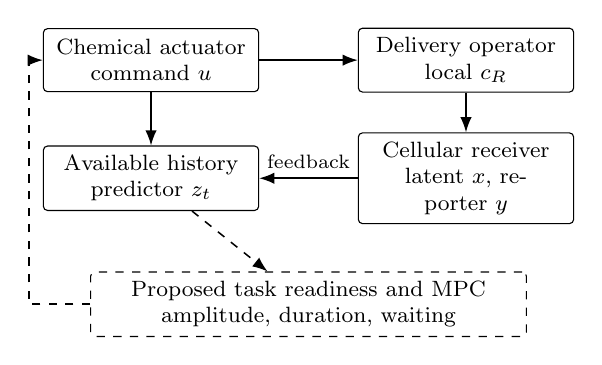
\begin{tikzpicture}[font=\footnotesize, >=Latex,
 box/.style={draw,rounded corners=1.5pt,align=center,minimum height=8mm,text width=25mm},
 arr/.style={->,line width=.55pt}]
\node[box] (act) at (0,1.5) {Chemical actuator\\command $u$};
\node[box] (del) at (4,1.5) {Delivery operator\\local $c_R$};
\node[box] (cell) at (4,0) {Cellular receiver\\latent $x$, reporter $y$};
\node[box] (hist) at (0,0) {Available history\\predictor $z_t$};
\node[box,dashed,text width=53mm] (mpc) at (2,-1.6) {Proposed task readiness and MPC\\amplitude, duration, waiting};
\draw[arr] (act) -- (del);
\draw[arr] (del) -- (cell);
\draw[arr] (cell) -- node[above,font=\scriptsize]{feedback} (hist);
\draw[arr] (act) -- (hist);
\draw[arr,dashed] (hist) -- (mpc);
\draw[arr,dashed] (mpc.west) -- (-1.55,-1.6) -- (-1.55,1.5) -- (act.west);
\end{tikzpicture}
\caption{MC interpretation and proposed feedback extension. The completed pilot predicts the reporter from commands and available observations. Local delivery, latent biochemical states, and the dashed task controller are not calibrated or implemented.}
\label{fig:system}
\end{figure}

\subsection{Task-Dependent Readiness: Proposed Definition}
A prospective command $m$ specifies an output band $\mathcal{Y}_m(t)$, a required hold interval, a completion deadline, and any exclusion interval for false activation. These values must come from a separately calibrated application. Let $\mathcal{I}_m$ contain the acquisition times in its required interval. At the resolution of the measurement system, task success is
\begin{equation}
 \begin{aligned}
 \mathcal{B}_m&=\bigcap_{t_i\in\mathcal{I}_m}\{y_j(t_i)\in\mathcal{Y}_m(t_i)\},\\
 S_m&=\ind\{\mathcal{B}_m\cap\mathcal{C}_m\}.
 \end{aligned}
 \label{eq:task}
\end{equation}
Here $\mathcal{C}_m$ is the event that the deadline and exclusion requirements are met. This definition makes no claim about unobserved behavior between frames. An individual-cell criterion differs from a population-mean criterion; the application must choose one before evaluating a policy. The present data have no prespecified $\mathcal{Y}_m$ or measured task labels, so Eq.~\eqref{eq:task} is not applied retrospectively to manufacture success rates.

For a candidate future command sequence $\mathbf a$, define readiness as
\begin{equation}
 R_t(m,\mathbf a)=\Prob(S_m=1\mid\Hist_t,\mathbf a).
 \label{eq:ready}
\end{equation}
Readiness is specific to a requested response and its deadline. Returning to a reporter baseline need not imply readiness for every next task. Conversely, successful delivery may not require complete biochemical reset. These are hypotheses to evaluate, not consequences of the current forecasting result. A point predictor and its RMSE do not provide a calibrated estimate of Eq.~\eqref{eq:ready}.

\section{Implemented History-Aware Predictor}
\subsection{Available Features}
We fit separate predictors for horizons $h=2$ and $10$ minutes. All learned predictors receive the same known future commanded waveform: its exposure in successive two-minute bins, the concentration at $t+h$, and the horizon. Future reporter values are targets only. This is conditional forecasting under a recorded protocol; it does not verify performance under arbitrary counterfactual commands.

The current-response feature set consists of $u_t$, $u_t^2$, $y_t$, $y_t^2$, $u_ty_t$, and the future-command features. A clock comparator additionally uses $t$ and $t^2$. A slope comparator uses the current features and $(y_t-y_{t-2})/2$, in reporter units per minute. The history model adds this causal slope, accumulated commanded exposure $\int_0^t u(s)\,ds$, and input/response filters with scales $\tau\in\{2,10,60\}$ minutes.

The input feature is the exact first-order response to the annotated piecewise-constant command:
\begin{equation}
 q_{\tau}(t)=\frac{1}{\tau}\int_0^t e^{-(t-s)/\tau}u(s)\,ds.
\end{equation}
For observation times $t_i$, the response feature satisfies
\begin{equation}
 r_{\tau,i}=e^{-\Delta_i/\tau}r_{\tau,i-1}
             +(1-e^{-\Delta_i/\tau})y_i,\quad
 r_{\tau,0}=y_0,
 \label{eq:ema}
\end{equation}
with $\Delta_i=t_i-t_{i-1}$. Prediction starts only after a fixed ten-minute observed warmup. Pre-export biological history remains unknown. The history model does not include the clock terms; comparison with the clock model is therefore not a fully nested history ablation. A history-plus-clock comparison is needed on new data.

\subsection{Condition-Weighted Ridge Learning}
Let $d$ index a training condition block, $N_d$ its forecast rows, and $D_{\rm tr}$ the number of such blocks. Each row receives weight $w_i=1/(D_{\rm tr}N_{d(i)})$, so the weights sum to one. Features are centered and scaled using weighted training means and standard deviations only. For standardized row $a_i$ and weighted target mean $\bar y$, the implemented fit is
\begin{equation}
 \hat\beta_{\lambda}=\arg\min_{\beta}
 \sum_{i\in\mathrm{train}}w_i
      (y_{i+h}-\bar y-a_i^\top\beta)^2
       +\lambda\|\beta\|_2^2.
 \label{eq:ridge}
\end{equation}
The intercept is $\bar y$ and is not penalized. Constant features are handled numerically by replacing a near-zero training scale with one. Ridge penalties are selected from $\{10^{-6},10^{-4},10^{-2},1,100\}$ by condition-equal validation MSE, separately for each predictor and horizon. Final coefficients are fit on training data; the validation blocks are not subsequently added to training.

Algorithm~1 summarizes the executed predictor. Its small feature set is intended to establish whether history carries useful information before selecting a more complex learning architecture. It is neither an inferred receptor-state model nor the MPC algorithm in the next section.

\begin{figure}[t]
\centering
\fbox{\begin{minipage}{.94\columnwidth}
\footnotesize
\textbf{Algorithm 1: Executed causal-history ridge predictor}\par\smallskip
\textbf{Input:} normalized cell trajectories, annotated command schedule, fixed condition split, horizon $h$.\par
1. Form rows after the ten-minute warmup; use only observations at or before $t$ for features.\par
2. Compute future-command bins, current features, slope, past exposure, and causal filters.\par
3. Estimate weighted scaling and target mean on training blocks.\par
4. For each candidate $\lambda$, fit Eq.~\eqref{eq:ridge} on training rows and score validation blocks equally.\par
5. Freeze the lowest-validation-error fit and predict mixed-protocol test rows once per saved fit.\par
\textbf{Output:} point forecasts and per-condition errors; no task-success probabilities or selected actions.
\end{minipage}}
\caption{Executed prediction algorithm. The test outputs have now been inspected; additional model development requires a new evaluation set.}
\label{alg:predictor}
\end{figure}

\section{Proposed Receiver-Reuse Controller}
\subsection{Planning Objective and Constraints}
The proposed extension uses an action $a_k=(A_k,d_k,w_k)$ comprising command amplitude, pulse duration, and waiting/washout duration. A finite sequence lies in $\calA$, the experimentally calibrated set of allowed sequences. The time for chemical washout and the time for cellular recovery can differ and should be measured separately. When cells share a chamber and one chemical command, the policy must optimize a prespecified population criterion, such as the fraction of eligible cells meeting the task; it cannot issue independent inputs to each tracked cell.

For ordered tasks $m_1,\ldots,m_K$, set $S_{\rm seq}=\prod_{k=1}^K S_{m_k}$. A candidate planning problem is
\begin{align}
 \min_{\mathbf a\in\calA}\quad &
  \eta_E\E[E(\mathbf a)\mid\Hist_t]
  +\eta_T\E[T(\mathbf a)\mid\Hist_t] \label{eq:mpc}\\
 \text{s.t.}\quad &
  \Prob(S_{\rm seq}=1\mid\Hist_t,\mathbf a)\geq1-\epsilon,
  \nonumber
\end{align}
with actuator bounds, task ordering, and deadlines included in $\calA$. The criterion concerns the joint sequence event. Multiplying marginal success probabilities would silently assume conditional independence and is not justified for a receiver reused across tasks.

The current concentration-time integral $E=\int u(t)\,dt$ is only an exposure proxy, with units ng$\cdot$min/ml. With calibrated flow $Q(t)$, delivered mass can instead be assessed as $\int Q(t)c_{\rm delivered}(t)\,dt$, with compatible units. Conversion to molecule number requires the molecular mass and an appropriate delivery model. No flow, delivered mass, or molecular savings are available in the present pilot.

\subsection{Learning and Online Operation to Be Implemented}
A future rollout model would predict a response distribution given $\Hist_t$ and a candidate waveform, using a mechanistic state estimator, a learned state model, or a learned residual to the mechanistic model. The ridge baseline does not select between these options. Distribution and task-event calibration must use separate data containing the relevant actions, histories, and outcomes; overlapping forecast residuals are not independent calibration trials.

Algorithm~2 is the proposed operational specification. A calibrated lower bound $\underline R_t$ may be used for the joint success constraint, but its construction and coverage must be validated under the intended deployment split. When no supported candidate meets the criterion, the experiment should retain its specified reference protocol or wait for another observation rather than interpret an uncalibrated forecast as evidence of feasibility. This behavior is a design requirement, not a verified guarantee.

\begin{figure}[t]
\centering
\fbox{\begin{minipage}{.94\columnwidth}
\footnotesize
\textbf{Algorithm 2: Proposed task-aware MPC (not executed)}\par\smallskip
\textbf{Prerequisites:} calibrated delivery, prespecified tasks, action-supported rollout model and joint-event calibration.\par
1. Update $\Hist_t$ with commands and feedback received by $t$.\par
2. Enumerate supported amplitude/duration/wait sequences in $\calA$ for the remaining ordered tasks.\par
3. Roll out response uncertainty; estimate joint sequence success and its calibrated lower bound $\underline R_t$.\par
4. Among sequences with $\underline R_t\geq1-\epsilon$ and satisfied deadlines, choose minimum exposure/time cost.\par
5. Execute only the first action, log actual actuation and delivery, and replan after feedback. If none qualifies, use the specified reference/wait rule.\par
\textbf{Output sought:} successful ordered tasks at reduced measured cost. No such output has yet been evaluated.
\end{minipage}}
\caption{Prospective control design. The probability model, calibration, optimizer, and online loop require implementation and new experiments.}
\label{alg:mpc}
\end{figure}

\section{Experimental Data and Evaluation Protocol}
\subsection{Source and Inventory}
The numerical files come from the paper-linked \texttt{Mijan/LFNS\_MSB} repository, using its MSB branch at pinned commit \texttt{5c917ab}; the full identifier is retained in the source manifest \cite{lfnsrepo}. All 47 saved source files were verified against their Git blob identifiers. The associated Mendeley record is cited for provenance \cite{mendeley2020}; the complete data archive and raw microscopy images were not downloaded. The pilot retains the authors' processed single-cell reporter trajectories and separate original-author simulation exports.

Table~\ref{tab:inventory} gives the eight condition blocks. Concentration amplitudes are 2.5 and 250 ng/ml. The data contain 606 cells and 53,998 observations at two-minute spacing. Sustained and periodic-pulse blocks span exported times 1--157 min; single-pulse blocks span 1--137 min; mixed blocks span 0--258 min. Independent experimental-day/session identifiers are unavailable. A block is a protocol--concentration grouping, not a verified independent biological replicate.

\begin{table}[t]
\caption{Experimental trajectory inventory and fixed split. Low/high denote 2.5/250 ng/ml; frames are per cell.}
\label{tab:inventory}
\centering\footnotesize
\begin{tabular}{llrrr}
\toprule
Partition & Protocol & Low $n$ & High $n$ & Frames \\
\midrule
Train & Sustained & 59 & 71 & 79 \\
Train & 3/20 pulses & 70 & 79 & 79 \\
Validation & Single 5-min & 88 & 85 & 69 \\
Test & Mixed pulses & 78 & 76 & 130 \\
\bottomrule
\end{tabular}

\end{table}

\subsection{Timing, Normalization, and Information Checks}
Commands follow the source model XML and the numerical pulse annotations, using half-open pulse intervals. Periodic stimulation applies three minutes on and twenty minutes off, with period 23 minutes. The single pulse spans $[0,5)$ min. Mixed pulses span $[1,4)$, $[24,54)$, and $[114,119)$ min relative to the export origin. The prose ordering of mixed-pulse durations differs from the executable annotations; we use the annotation/XML agreement and retain that discrepancy in the audit.

For the mixed condition, we reconstructed normalization from unnormalized exports using the original 10--30 minute per-cell median baseline, before the origin shifted by 42 minutes. The maximum reconstruction discrepancy was $1.40\times10^{-4}$ and $1.35\times10^{-4}$ for low and high concentration, consistent with export rounding. The baseline therefore precedes the evaluated forecast history. Other conditions retain author preprocessing and have not undergone a complete raw-image-to-reporter reconstruction. Claims of online causality are conditional on these processed measurements.

Population means were recomputed from individual exported cells. The largest difference from an author-provided mean was $5.64\times10^{-4}$, in the sustained high-dose block. We use the recomputed means consistently. Feature-prefix checks verify that future reporter values do not enter forecast features or their training scaling; these software checks cannot certify unrecorded aspects of the original microscopy preprocessing.

\subsection{Scores and Comparators}
The primary score is the square root of the equally weighted condition MSE:
\begin{equation}
 \mathrm{RMSE}_{\rm cond}(h)=
 \left[\frac{1}{|D_{\rm te}|}\sum_{d\in D_{\rm te}}
 \frac{1}{N_{d,h}}\sum_{i\in d}(\hat y_{i+h}-y_{i+h})^2\right]^{1/2}.
 \label{eq:score}
\end{equation}
Here $|D_{\rm te}|=2$. After warmup and horizon eligibility, there are 19,096 two-minute forecast rows and 18,480 ten-minute rows. These overlapping rows and cells are not independent intervention replicates, so no independent-day confidence interval or significance test is reported. The split is fixed across predictors, but the pilot test has now been viewed and cannot serve as an untouched test for future method selection.

We compare persistence, current input, current response, current response plus clock, current response plus slope, and causal history. For a separate open-loop diagnostic, a positive single-lag model and a regularized stable filter bank predict population means without reporter feedback. The single-lag time constant is selected on validation from 100 logarithmic candidates between 0.2 and 200 min, with nonnegative dose-specific gains fit on training blocks. The bank uses scales 1, 2, 4, 8, 16, 32, 64, and 128 min and training/validation ridge selection. These are phenomenological command-to-reporter models, not calibrated transport or receptor models.

Finally, we show the mean of 1,000 predictive samples exported for the source authors' B3 biochemical model. Its architecture selection used mixed and single-pulse conditions, so it is a selection-exposed contextual reference. It was not refit here and is not a fresh blind test. Population-mean open-loop errors must not be compared as if they were the individual-cell, observation-feedback forecast errors in Eq.~\eqref{eq:score}.

\section{Results}
\subsection{Protocol-Held-Out Reporter Prediction}
Table~\ref{tab:forecast} reports all six predictors. The history predictor has the lowest point RMSE among these tested models at both horizons. At 10 min, its RMSE is 0.026817 versus 0.029597 for current input/response and 0.029229 for current input/response/clock, corresponding to 9.39\% and 8.25\% relative reductions. At 2 min, its improvement over current input/response is only 0.94\%. This pattern supports studying history for longer prediction horizons while limiting any practical interpretation of the short-horizon gain.

\begin{table}[t]
\caption{Condition-equal test RMSE of individual-cell forecasts, in normalized reporter units. Bold indicates the smallest point estimate, without an independent-day uncertainty claim.}
\label{tab:forecast}
\centering\footnotesize
\begin{tabular}{lrrrrr}
\toprule
Predictor & 2 min & 10 min & Val. & $\le$147 & $>$147 \\
\midrule
Persistence & 0.01588 & 0.03105 & 0.02492 & 0.03698 & \textbf{0.02047} \\
Input only & 0.04602 & 0.04598 & 0.04400 & 0.04725 & 0.04422 \\
Input+response (IR) & 0.01554 & 0.02960 & 0.02611 & 0.03364 & 0.02302 \\
IR + clock & 0.01560 & 0.02923 & 0.02648 & 0.03354 & 0.02209 \\
IR + slope & 0.01586 & 0.02958 & 0.02591 & 0.03386 & 0.02253 \\
Causal history & \textbf{0.01539} & \textbf{0.02682} & \textbf{0.02453} & \textbf{0.03060} & 0.02062 \\
\bottomrule
\end{tabular}

\end{table}

All learned models with response feedback select $\lambda=10^{-6}$; the current-input-only model selects $\lambda=100$ at both horizons. The ten-minute per-condition history MSE is 0.000814 at low dose and 0.000624 at high dose, compared with 0.000930 and 0.000779 for the clock comparator. The direction of the point improvement is thus shared by both tested concentration blocks. These blocks do not establish robustness across experimental days or generalization to unseen concentration amplitudes.

\begin{figure}[t]
\centering
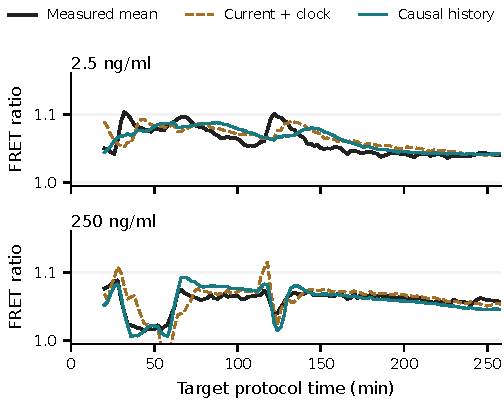
\includegraphics[width=\columnwidth]{figures/forecast_mean_10min.pdf}
\caption{Ten-minute forecasts averaged across test cells at each target time. Each prediction uses that cell's observations only up to its forecast origin. Curves aid interpretation; Table~\ref{tab:forecast} scores individual-cell errors, not these averaged curves.}
\label{fig:forecast}
\end{figure}

\subsection{Command-Only Models and Washout Behavior}
Fig.~\ref{fig:mixed} shows the measured mixed-protocol mean, phenomenological models, and B3 reference. The fitted positive single-lag constant is 13.16 min, with gains 0.1025 and 0.0477 at low and high concentration. For the full 0--258 min test window, its condition-equal population-mean RMSE is 0.054101; the heavily regularized stable bank gives 0.021493. The bank stays close to an average level and does not reconstruct the principal pulse-dependent features well. These fits do not reveal physical diffusion, flow, receptor, or reaction-rate parameters.

\begin{figure*}[t]
\centering
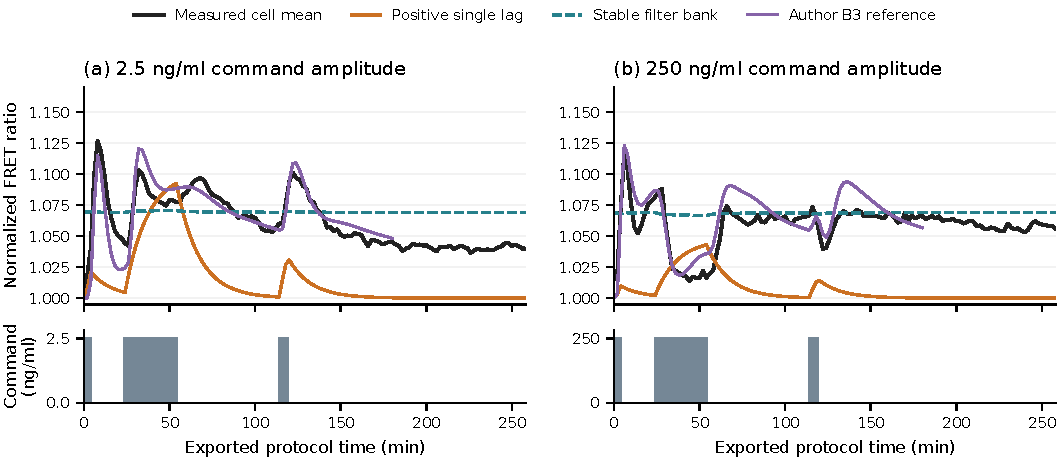
\includegraphics[width=.97\textwidth]{figures/mixed_response.pdf}
\caption{Mixed-protocol cell means and open-loop command-to-reporter models, with commanded pulses below. The B3 line is the original authors' predictive mean and ends at 180 min. Its architecture-selection exposure makes it a contextual reference, not a blind benchmark. No local-concentration trace is available.}
\label{fig:mixed}
\end{figure*}

On the common 0--180 min window, Table~\ref{tab:openloop} shows that the source B3 reference is closer to the population mean than either simple command-only model. This observation argues for a serious biochemical comparator in subsequent work. It does not prove that a mechanistic controller outperforms a learned controller, since no such policies were tested with matched feedback.

\begin{table}[t]
\caption{Population-mean open-loop RMSE on 0--180 min. B3 is selection-exposed and receives a different information/evaluation setup from the individual-cell forecasts.}
\label{tab:openloop}
\centering\footnotesize
\begin{tabular}{lrr}
\toprule
Population-mean model & 2.5 ng/ml & 250 ng/ml \\
\midrule
Positive single lag & 0.05395 & 0.05675 \\
Stable filter bank & 0.02071 & 0.02245 \\
Training-mean constant & 0.02091 & 0.02306 \\
Author B3 reference & 0.01146 & 0.01362 \\
\bottomrule
\end{tabular}

\end{table}

In an illustrative washout contrast chosen after waveform inspection, the mean reporter increases from 1.077330 to 1.095792 between 54 and 66 min at low dose, and from 1.016545 to 1.074167 at high dose. The within-cell increases are positive for 58/78 and 73/76 cells, respectively. The command is zero throughout this interval. A nonnegative single-lag command-driven state must decay toward baseline while its input is zero, so it cannot reproduce this increase. However, the local concentration is unobserved: this diagnostic cannot assign the mismatch uniquely to intracellular memory rather than delivery or measurement dynamics. The source biology already reports complex washout behavior \cite{blum2019}.

\subsection{Exploratory Matched-History Analysis}
To examine whether similar present measurements can precede different future responses, we compare early washout after the short pulse ($t=6$--12 min) with later washout after the long pulse ($t=56$--102 min), within the same cell. Both candidate times have zero commanded exposure for the next ten minutes. One pair per cell is selected by minimum current-reporter discrepancy, with tolerance 0.005. A stricter analysis also limits causal-slope discrepancy to 0.002 reporter units/min. Future outcomes are not used to select pairs, but the time windows and matching rule were chosen after viewing the data.

Table~\ref{tab:matching} reports the mean later-minus-earlier ten-minute target. At low dose, the difference is positive in both matching variants. At high dose, the current-only difference is negative and shrinks to $-0.001213$ after slope matching; only 17/76 cells then remain. The result is not a consistent, concentration-independent demonstration of additional hidden history information.

\begin{table}[t]
\caption{Exploratory within-cell history matching. Dose is in ng/ml; $\overline{\Delta y_{+10}}$ is the later-minus-earlier target mean. Sparse support and post hoc choices limit interpretation.}
\label{tab:matching}
\centering\footnotesize
\begin{tabular}{lcrr}
\toprule
Dose & Matched features & Cells & $\overline{\Delta y_{+10}}$ \\
\midrule
2.5 & $y$ & 60/78 & +0.014404 \\
2.5 & $y$, slope & 14/78 & +0.020186 \\
250 & $y$ & 69/76 & -0.015529 \\
250 & $y$, slope & 17/76 & -0.001213 \\
\bottomrule
\end{tabular}

\end{table}

Within-cell matching holds cell identity fixed but does not hold cellular age, protocol time, unmeasured physiological state, or local delivery fixed. Conditioning on a post-stimulation reporter also does not identify a controlled direct effect of prior exposure. Regression to the mean and selection on common support remain possible. These contrasts motivate prospective preconditioning experiments; they supply neither a causal memory estimate nor evidence of a newly discovered pathway mechanism.

\section{Discussion and Required Validation}
\subsection{What Makes the Question Molecular}
The proposed task requires nonnegative chemical actuation, delivery and washout dynamics, a nonlinear cellular receiver, and history-dependent response availability. Waiting is a potentially useful control action with a completion-time cost; chemical exposure has its own cost. A receiver may continue responding when the actuator has stopped, and a reporter measurement may fail to reveal the full state required for the next command. These properties determine the optimization variables and evaluation target. Replacing a wireless waveform with an arbitrary fluorescence array would not establish them.

The pilot does not separate delivery memory from receptor or intracellular memory, infer a biochemical state, or measure functional cell fate. It provides an initial data-grounded response predictor. Any broader application claim requires calibrating the link and the response task, not merely increasing forecasting accuracy.

\subsection{Prospective Experiments}
A decisive next experiment should randomize short versus long preconditioning at the independent chamber/session level, counterbalance protocol time and cell age, and then administer a common second command after candidate waits. The present plan lists 6, 12, 24, and 48 min waits and a five-minute probe as pilot candidates; they are not optimized settings. Local concentration, flow, actual actuation timestamps, reporter quality, feedback arrival time, and complete failures must be logged. Task bands, hold times, deadlines, and false-activation criteria must be fixed on separate calibration data before formal evaluation.

The central test concerns at least two ordered commands. Compare fixed waiting, reporter-threshold reset, a B3-based state estimator and MPC, present-response/slope/clock learning, and history-plus-clock learning. All adaptive methods must receive the same observations, future-command information, action bounds, and uncertainty-calibration budget. A learned residual is justified only if it adds reproducible value beyond the biochemical estimator. Comparison should measure exposure or delivered mass and completion time at matched sequence reliability, including unsuccessful sequences.

Randomized preconditioning tests the total effect of prior chemical exposure. Comparing prognostic models within overlapping present-state support tests whether the extra history improves prediction; it does not, by itself, identify a direct causal history effect after fixing the present reporter. New experimental-day splits are needed for both questions. The number of cells or rolling forecast windows cannot replace independent intervention units when choosing sample size or uncertainty estimates.

\subsection{Interpretation and Novelty Threshold}
The current evidence is a modest protocol-held-out learning result. The two-minute benefit is small, the clock comparison is not a fully nested ablation, and the high-dose slope-matched contrast weakens a simple hidden-memory narrative. A trained neural model, task probability calibration, live controller, dose saving, and repeated-command success have not been demonstrated. Offline replay of these open-loop traces cannot reliably evaluate actions that were never executed.

The intended stronger contribution would be a reproducible sequence-level cost reduction caused by usable receiver-history information, after transport calibration and comparison with matched-feedback biochemical control. That outcome would substantiate a specific advance in MC operation. If history adds no independent-day benefit, or if the mechanistic estimator reaches the same reliability and cost, the claim should be narrowed accordingly. Targeted full-text gaps and relevant supplements must also be closed before making a priority claim.

\balance
\section{Conclusion}
We implemented a transparent history-aware predictor on experimentally measured FGF2--ERK trajectories with a fixed condition-level split and auditable sources. The best tested history baseline reduces ten-minute RMSE by 8.25\% relative to a current-input/current-response/clock comparator, while the short-horizon gain is small and exploratory matching does not consistently establish an additional history effect. We formulate task-dependent readiness and a prospective receding-horizon controller for repeated use of a cellular receiver. Demonstrating this controller's value requires calibrated delivery, prespecified tasks, supported interventions, and new independent-session experiments. The present manuscript is a data-grounded starting point for that validation, not evidence of an already established pioneering control result.

\section*{Data and Code Availability}
The accompanying source package includes the manuscript, vector plots, asset-generation script, frozen numerical results, reproducible pilot code, source manifest, targeted novelty audit, and proposed experimental configuration. Numerical sources are credited in \cite{blum2019,lfnsrepo,mendeley2020}; original-author files retain their attribution and are assigned no new license. The included asset script rebuilds tables and plots without fitting or retuning models. Full preprocessing, limitations, and reproduction commands are documented in the package.

\bibliographystyle{unsrt}
\bibliography{references}
\end{document}
